
\documentclass{ctexart}
\usepackage{graphicx}
\usepackage{booktabs}
\usepackage{multirow}
\usepackage{subfigure}

\begin{document}
\label{chap:testlk}
中文测试,通过该文档检测中文在latex中的输入是否有问题,在ubuntu14.04中测试效果
$\alpha$ , $\beta$  and ,$\gamma$

\begin{equation}
\label{eq:1}
f(x)=ax^2+bx+c
\end{equation}


$\alpha$

$\sigma$
$\Sigma$
$\epsilon$
$\lambda$


\[\sigma^{2}=\frac{1}{N}\sum_{n=1}^{N}(x_n-y_n)^{2}]



$\cos$
\begin{equation}{2.0} 
\label{eq:3}

\end{equation}



$a\tilde{\cos\Gamma\}$

f(y)=ay^3+by^2+c
\begin{spacing}{}

\end{environment}
\begin{center}


the quick brown dog  over the lazy fox 0 1 2 3.1459 4 5 6 7 8 9 times
the quick brown dog  over the lazy fox 0 1 2 3.1459 4 5 6 7 8 9 times
the quick brown dog  over the lazy fox 0 1 2 3.1459 4 5 6 7 8 9 times
\end{center}

the quick brown dog  over the lazy fox 0 1 2 3.1459 4 5 6 7 8 9
timesthe quick brown dog  over the lazy fox 0 1 2 3.1459 4 5 6 7 8 9
times
the quick brown dog  over the lazy fox 0 1 2 3.1459 4 5 6 7 8 9 times
the quick brown dog  over the lazy fox 0 1 2 3.1459 4 5 6 7 8 9 times
the quick brown dog  over the lazy fox 0 1 2 3.1459 4 5 6 7 8 9 times
the quick brown dog  over the lazy fox 0 1 2 3.1459 4 5 6 7 8 9 times
the quick brown dog  over the lazy fox 0 1 2 3.1459 4 5 6 7 8 9 times
the quick brown dog  over the lazy fox 0 1 2 3.1459 4 5 6 7 8 9 times
\end{spacing}




ref for the test
\left\gamma{}

\begin{math}
  test math ax^5
\end{math}

\section{section1}
\label{sec:文字输入测试}





\section{section2}
\label{sec:公式测试}

fig:



\ldots this is an formular:
\begin{equation}
  \label{eq:2}
   \sum _{k=1} ^{n}I_k=0 \; .
\end{equation}

\begin{displaymath}
 
\begin{aligned}
\label{eq:4}
&NU^{+}=\rho_{1}+\rho_{2}+\frac{\rho_{3}}{3} \\
&NU=\rho_{1}+\frac{\rho_{3}}{2} \\
\end{aligned}
\end{displaymath}


\begin{displaymath}
\mathbf{X} =
\left(\begin{array}{c|c|c}

NU^{+}=\rho_{1}&\rho_{2}&\frac{\rho_{3}}{3} \\
NU=\rho_{1}&0&\frac{\rho_{3}}{2} \\
\end{array} \right)

\end{displaymath}



\begin{eqnarray}
\label{eq:5}
NU^{+}=\rho_{1}+\rho_{2}+\frac{\rho_{3}}{3} \\
NU=\rho_{1}+\frac{\rho_{3}}{2} 
\end{eqnarray}


\section{section3}
\label{图形测试}
\begin{figure}[htbp]
\centerline{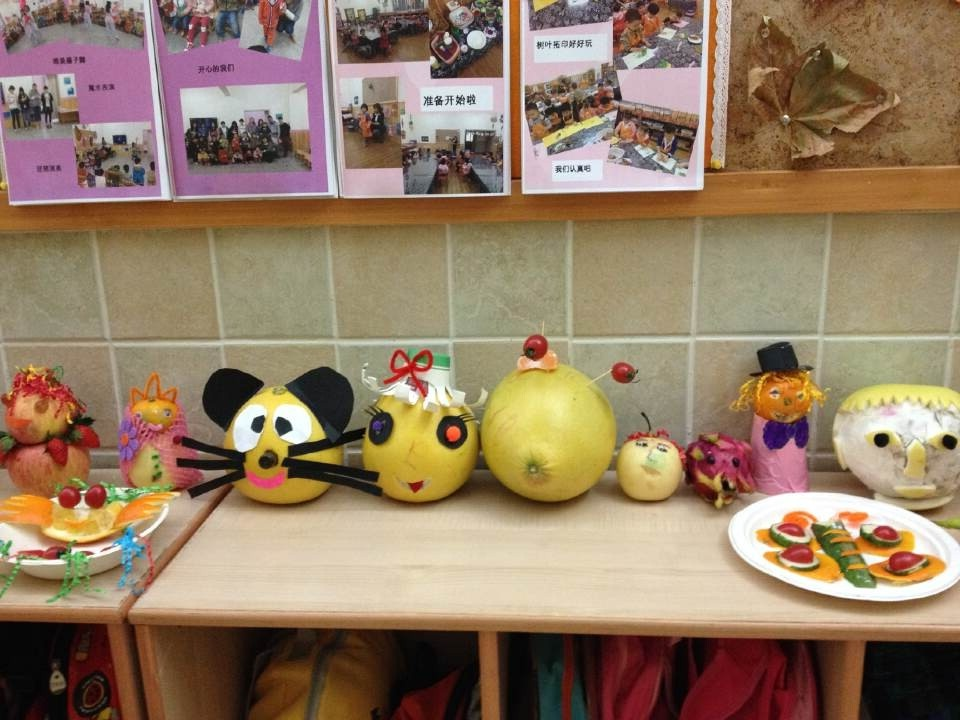
\includegraphics[width=1.77in,angel=90]{test2.eps}}
\caption[]{测试图片\label{fig:test2} }
\end{figure}

\begin{figure}[htbp]
\centerline{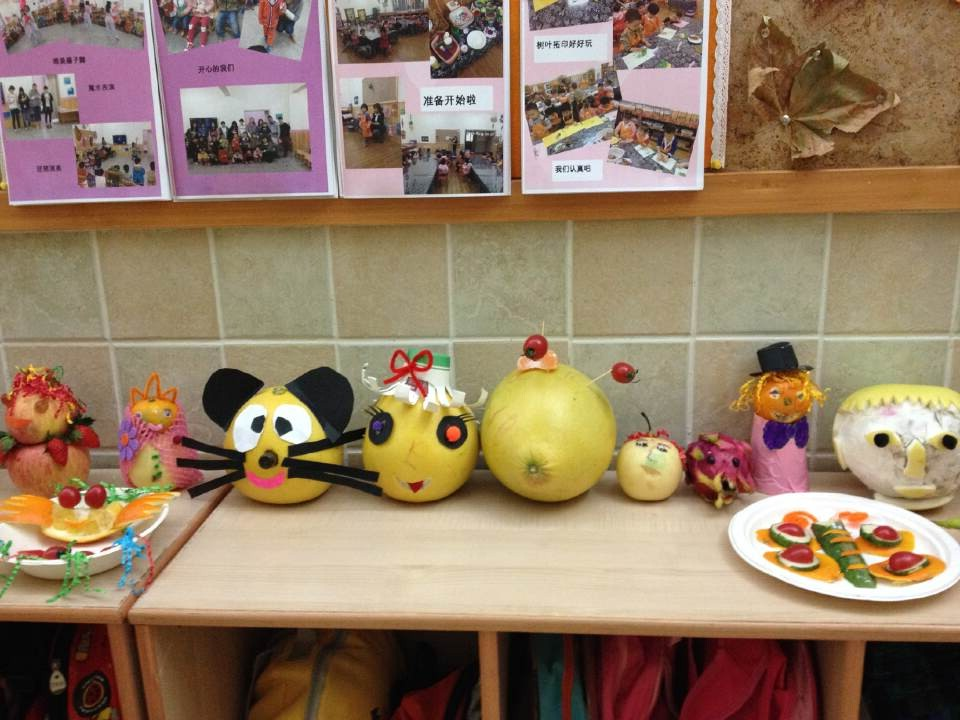
\includegraphics[width=3in,angel=90]{test.jpg}}
\caption[test2]{测试图片test\label{fig:testjpg} }
\end{figure}

\begin{figure}[htbp]

\subfigure[fig(a)]
{\label{fig:subfig:a}
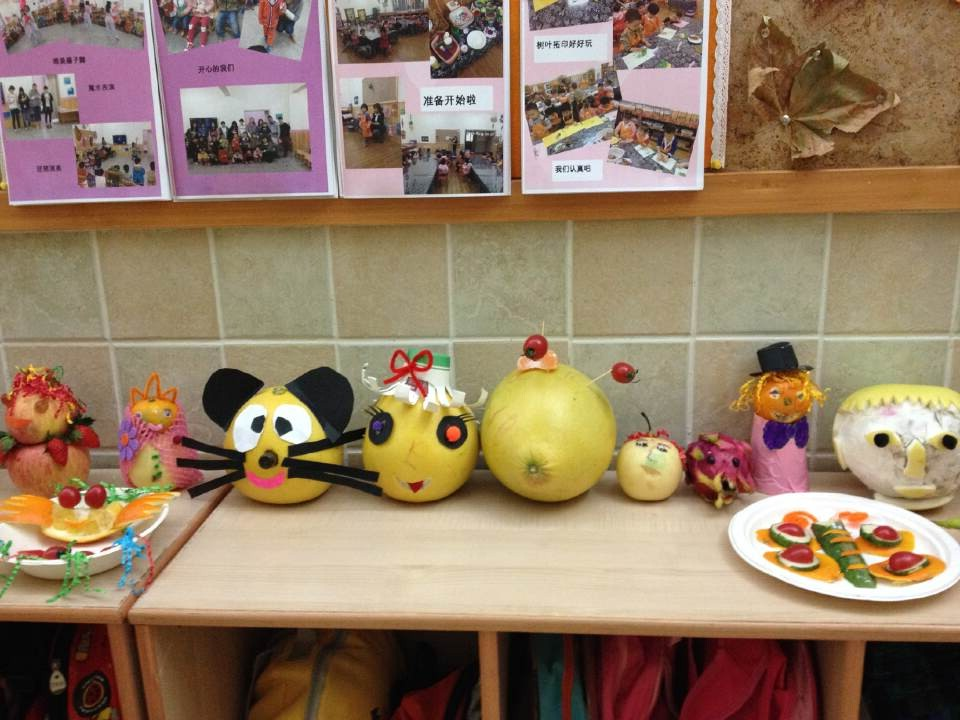
\includegraphics[width=1.5in]{test.jpg}}

\subfigure[subfigure2]
{\label{fig:subfig:b}
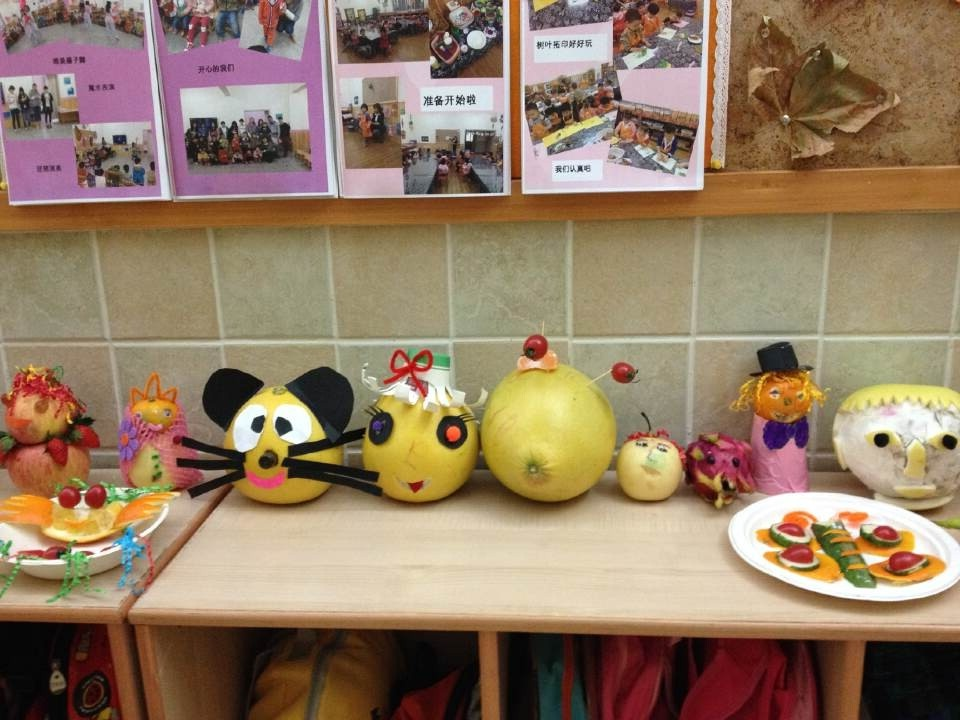
\includegraphics[width=1.5in]{test2.jpg}}

\caption[]{\label{fig:subfigure} }
\end{figure}


test\cite{rowe-1979-grain}



\begin{tabular}{|l|c|r|c|}
 \hline
操作系统& 发行版& 编辑器 &备注\\
 \hline
Windows & MikTeX & TexMakerX &测试1 \\
 \hline
Unix/Linux & teTeX & Kile  &测试2 \\
 \hline
Mac OS & MacTeX & TeXShop  &测试3\\
 \hline
通用& TeX Live & TeXworks  &测试4\\
 \hline
\end{tabular}


LaTeX table example\\
\verb= http:\\www.chinatex.org=\\
\begin{table}[!hbp]
\begin{tabular}{|c|c|c|c|c|}
\hline
lable 1-1 & label 1-2 & label 1-3 & label 1 -4 & label 1-5 \\
\hline
label 2-1 & label 2-2 & label 3-3 & label 4-4 & label 5-5 \\
\hline
\multirow{2}{*}{Multi-Row} & \multicolumn{2}{|c|}{Multi-Column} & \multicolumn{2}{|c|}{\multirow{2}{*}{Multi-Row and Col}} \\
\cline{2-3}
& column-1 & column-2 & \multicolumn{2}{|c|}{}\\
\hline
\end{tabular}
\caption{My first table}
\end{table}





\begin{table}
\begin{tabular}{|c|c|c|}
\toprule
姓名& 学号& 性别\\
\midrule
Ch'en Meng& 001& Male\\
Sarah Brightman& 002& Female\\
\bottomrule
\end{tabular}
\end{table}



\section{section4}
\label{参考文献测试}
\la
tes

testcite\cite{Murray2009hydrogen}the new document

\begin{equation}
3 \cite{kraus}
4\cite{test-new}
5\cite{landau}
6\cite{Balkan:2017:UFA:3136518.3122787}
7\cite{Schedl:2016:IIM:3004291.2991468}
8\cite{Han:2016:TUB:2992189.2992202}\cite{Crowston:2017:GSH:3022198.3026329}

yinyong\cite{Larochelle:2012:LAC:2188385.2188407}

\begin{equation}


\bibliographystyle{unsrt}
\bibliography{name}



\end{document}
